\begin{titlepage}
\begin{center}

\includegraphics[scale=0.15]{Documents/niser.png}
\line(1,0){300}\\
[2mm]
\begin{large}
\textbf{\huge Phase Shift Oscillator}\\ 
\end{large}
\line(1,0){150}\\
[5cm]
\large MAITREY SHARMA\\
\small (1911093)\\
[4.5cm]
Second Year Integrated M.Sc.\\
\textbf{School of Physical Sciences}\\
\textbf{National Institute of Science Education and Research, Bhubaneshwar}\\
\small March 10, 2021
\end{center} 
\end{titlepage}
\newpage
\section{Aim}
\noindent To construct and determine the resonant frequency of a phase shift oscillator.
\section{Apparatus}
\noindent Op-Amp IC741, resistors, oscilloscope, DC voltage source, function generator, digital storage oscilloscope, breadboard, multimeters and connecting wires.
\section{Theory}
\noindent An \textbf{\emph{electronic oscillator}} is an electronic circuit that produces a periodic, oscillating electronic signal, often a sine wave or a square wave or a triangle wave. Oscillators convert direct current (DC) from a power supply to an alternating current (AC) signal. 
\begin{center}
    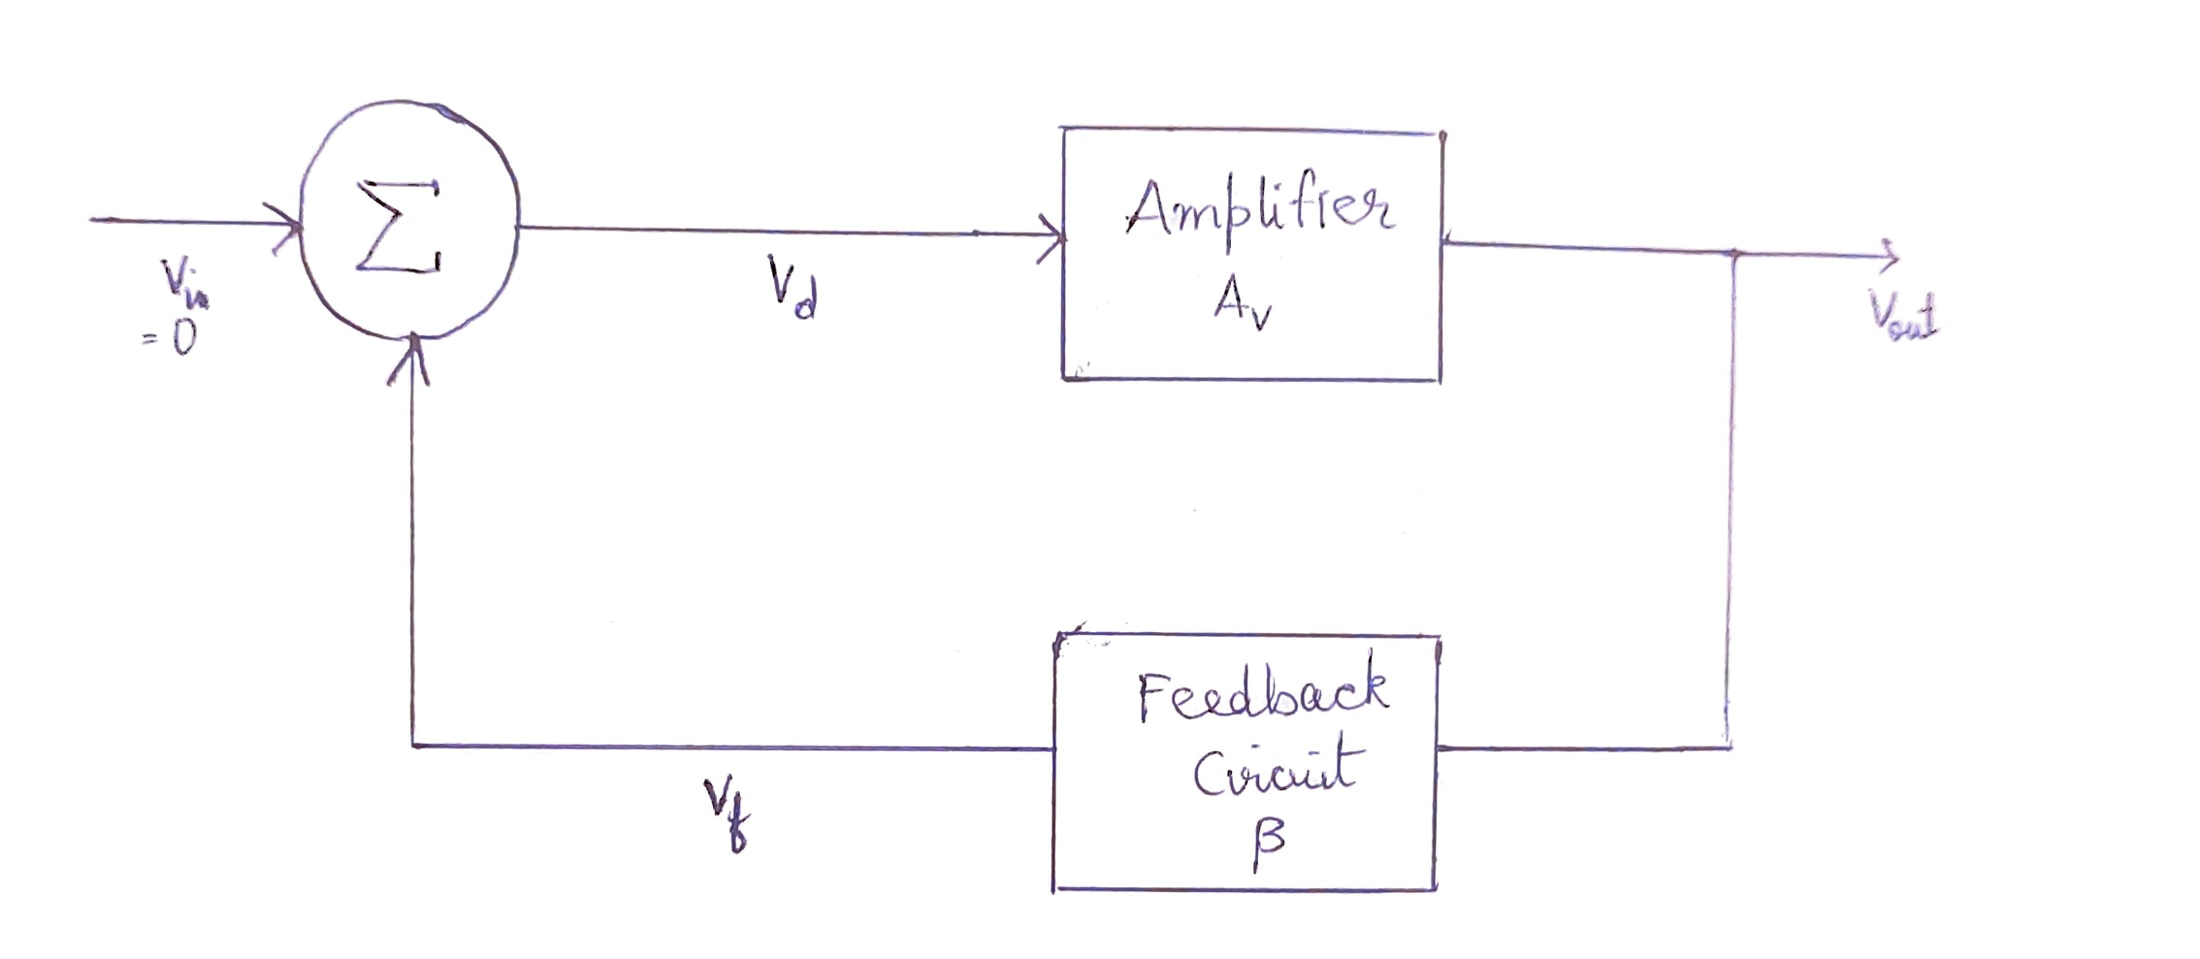
\includegraphics[scale = 0.22]{Documents/block.jpg}
\end{center}
\begin{center}
    \textbf{Fig 3.1 Block diagram of an oscillator}
\end{center}
\noindent
From the block diagram, 
\begin{center}
    $V_d = V_f + V_{in}$; $V_o = A_v V_d$; $V_f = \beta V_o$
\end{center}
\noindent From here, 
\begin{center}
    $\dfrac{V_o}{V_{in}} = \dfrac{A_v}{1 - A_v \beta }$
\end{center}
\par
\noindent
The \textbf{\emph{Barkhausen stability criterion}} is a mathematical condition to determine when a linear electronic circuit will oscillate. It states that if $A_v$ is the gain of the amplifying element in the circuit and $\beta$ is the transfer function of the feedback path, so $A_v \beta$ is the loop gain around the feedback loop of the circuit, the circuit will sustain steady-state oscillations only at frequencies for which:
\begin{enumerate}
    \item The loop gain is equal to unity in absolute magnitude, that is, $|A_v \beta| = 1$ and
    \item The phase shift around the loop is zero or an integer multiple of $2 \pi$, that is, $\angle \beta A_v = 2 \pi n, n \in \{0, 1, 2, ...\}$
\end{enumerate}
\bigskip
\par
\noindent
A \textbf{\emph{phase-shift oscillator}} is a linear electronic oscillator circuit that produces a sine wave output. The phase-shift oscillator designed here consists of an Op-Amp as an \emph{inverting amplifier element} with its output fed back to its input through a phase-shift network consisting of resistors and capacitors in a \emph{ladder network}. The feedback network \emph{shifts} the phase of the amplifier output by 180 degrees at the oscillation frequency to give \textbf{\emph{positive feedback}}.
\newline
\noindent
The construction of the circuit of the phase-shift oscillator consists of an Op-Amp as the amplifying stage and three RC cascaded networks as the feedback circuit. The Op-Amp used in this oscillator is in the inverting mode, output is $180 \degree$ is phase shifted.
\begin{center}
    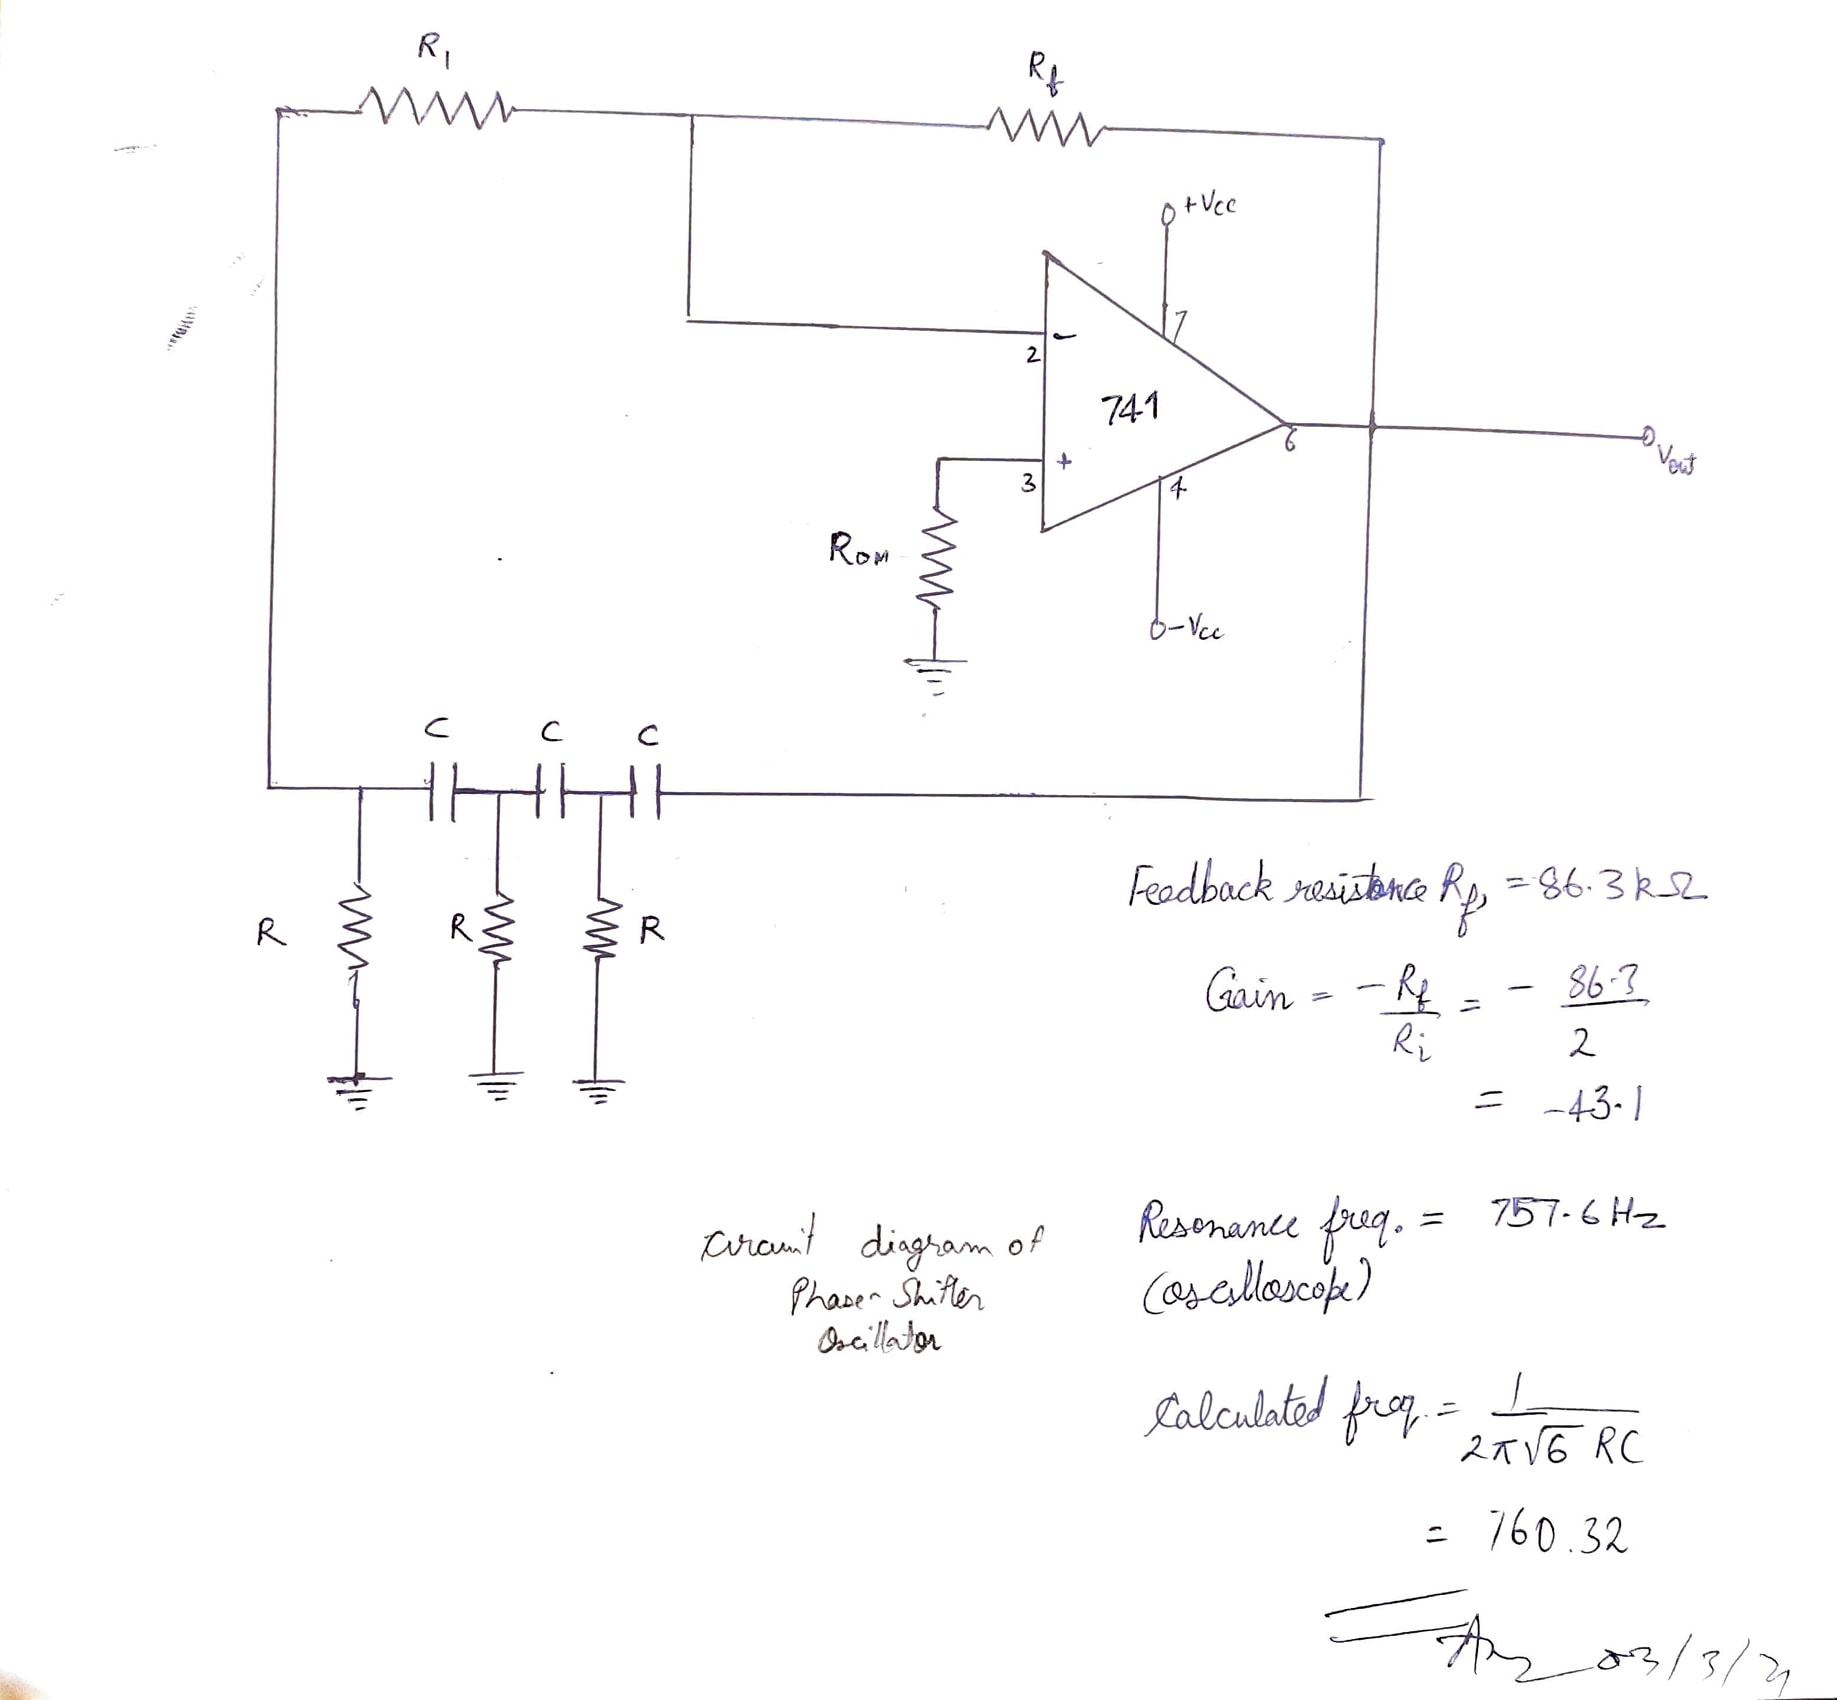
\includegraphics[scale = 0.25]{Documents/pso.jpg}
\end{center}
\begin{center}
    \textbf{Fig 3.2 Circuit diagram used for the experiment}
\end{center}
\noindent We can analyse the circuit for a general case as well. Consider the following implementation of the phase-shift oscillator shown in the diagram (Fig 3.3) uses an Op-Amp, three capacitors and four resistors.
\begin{center}
    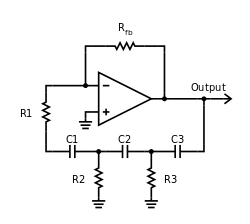
\includegraphics[scale = 0.85]{Documents/wikirc.png}
\end{center}
\begin{center}
    \textbf{Fig 3.3 A general circuit for phase-shift oscillator}
\end{center}
For this particular circuit, assuming an ideal amplifier, the oscillation frequency is:
\begin{center}
    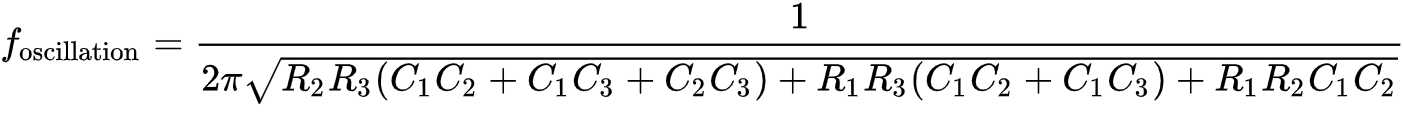
\includegraphics[scale = 0.4]{Documents/foscc.png}
\end{center}
and the feedback resistance required to sustain the oscillations is:
\begin{center}
    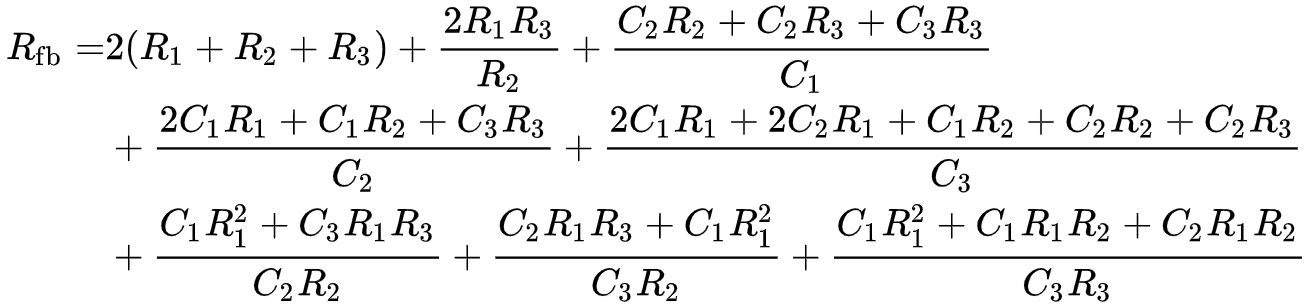
\includegraphics[scale = 0.4]{Documents/rfb.png}
\end{center}
If here, $R_1 = R_2 = R_3 = R$ and $C_1 = C_2 = C_3 = C$ then the the expressions reduce to:
\begin{center}
    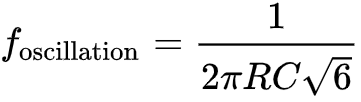
\includegraphics[scale = 0.4]{Documents/redfoscc.png}
\end{center}
\begin{center}
    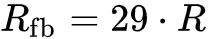
\includegraphics[scale = 0.4]{Documents/redrfb.png}
\end{center}
Thus, the feedback circuit with RC network gives $180 \degree$ phase shift but decreases the output 
voltage by a factor of 29. That is, $\beta = 1/29$. For oscillations, $A_v \beta = 1$. Therefore, gain 
should be at least 29.
\clearpage
\noindent
A \textbf{\emph{Lissajous figure}} is the graph of the system of the parametric equations:
\begin{center}
    $x = A sin(at + \delta), y = B sin(bt)$
\end{center}
which describe complex harmonic motion. The result of sustained oscillations is the formation of a Lissajous figure which is circular/elliptical.
\section{Observations}
\begin{enumerate}
    \item $R_f = \SI{86.3}{k \ohm}$ (obtained using the potentiometer). 
    \item $R_1 = r_a + r_b = \SI{0.990}{k\ohm} + \SI{0.996}{k \ohm}$
    \item $R = \SI{1.011}{k\ohm}, \SI{0.991}{k \ohm}, \SI{0.984}{k \ohm}$.
    \item $C = \SI{78.0}{n \farad}, \SI{104.2}{n \farad}, \SI{103.3}{n \farad}$
    \item $A_v = |\dfrac{R_f}{R_1}| = 43.45 > 29$ (sustained oscillations will take place)
\end{enumerate}
\begin{center}
    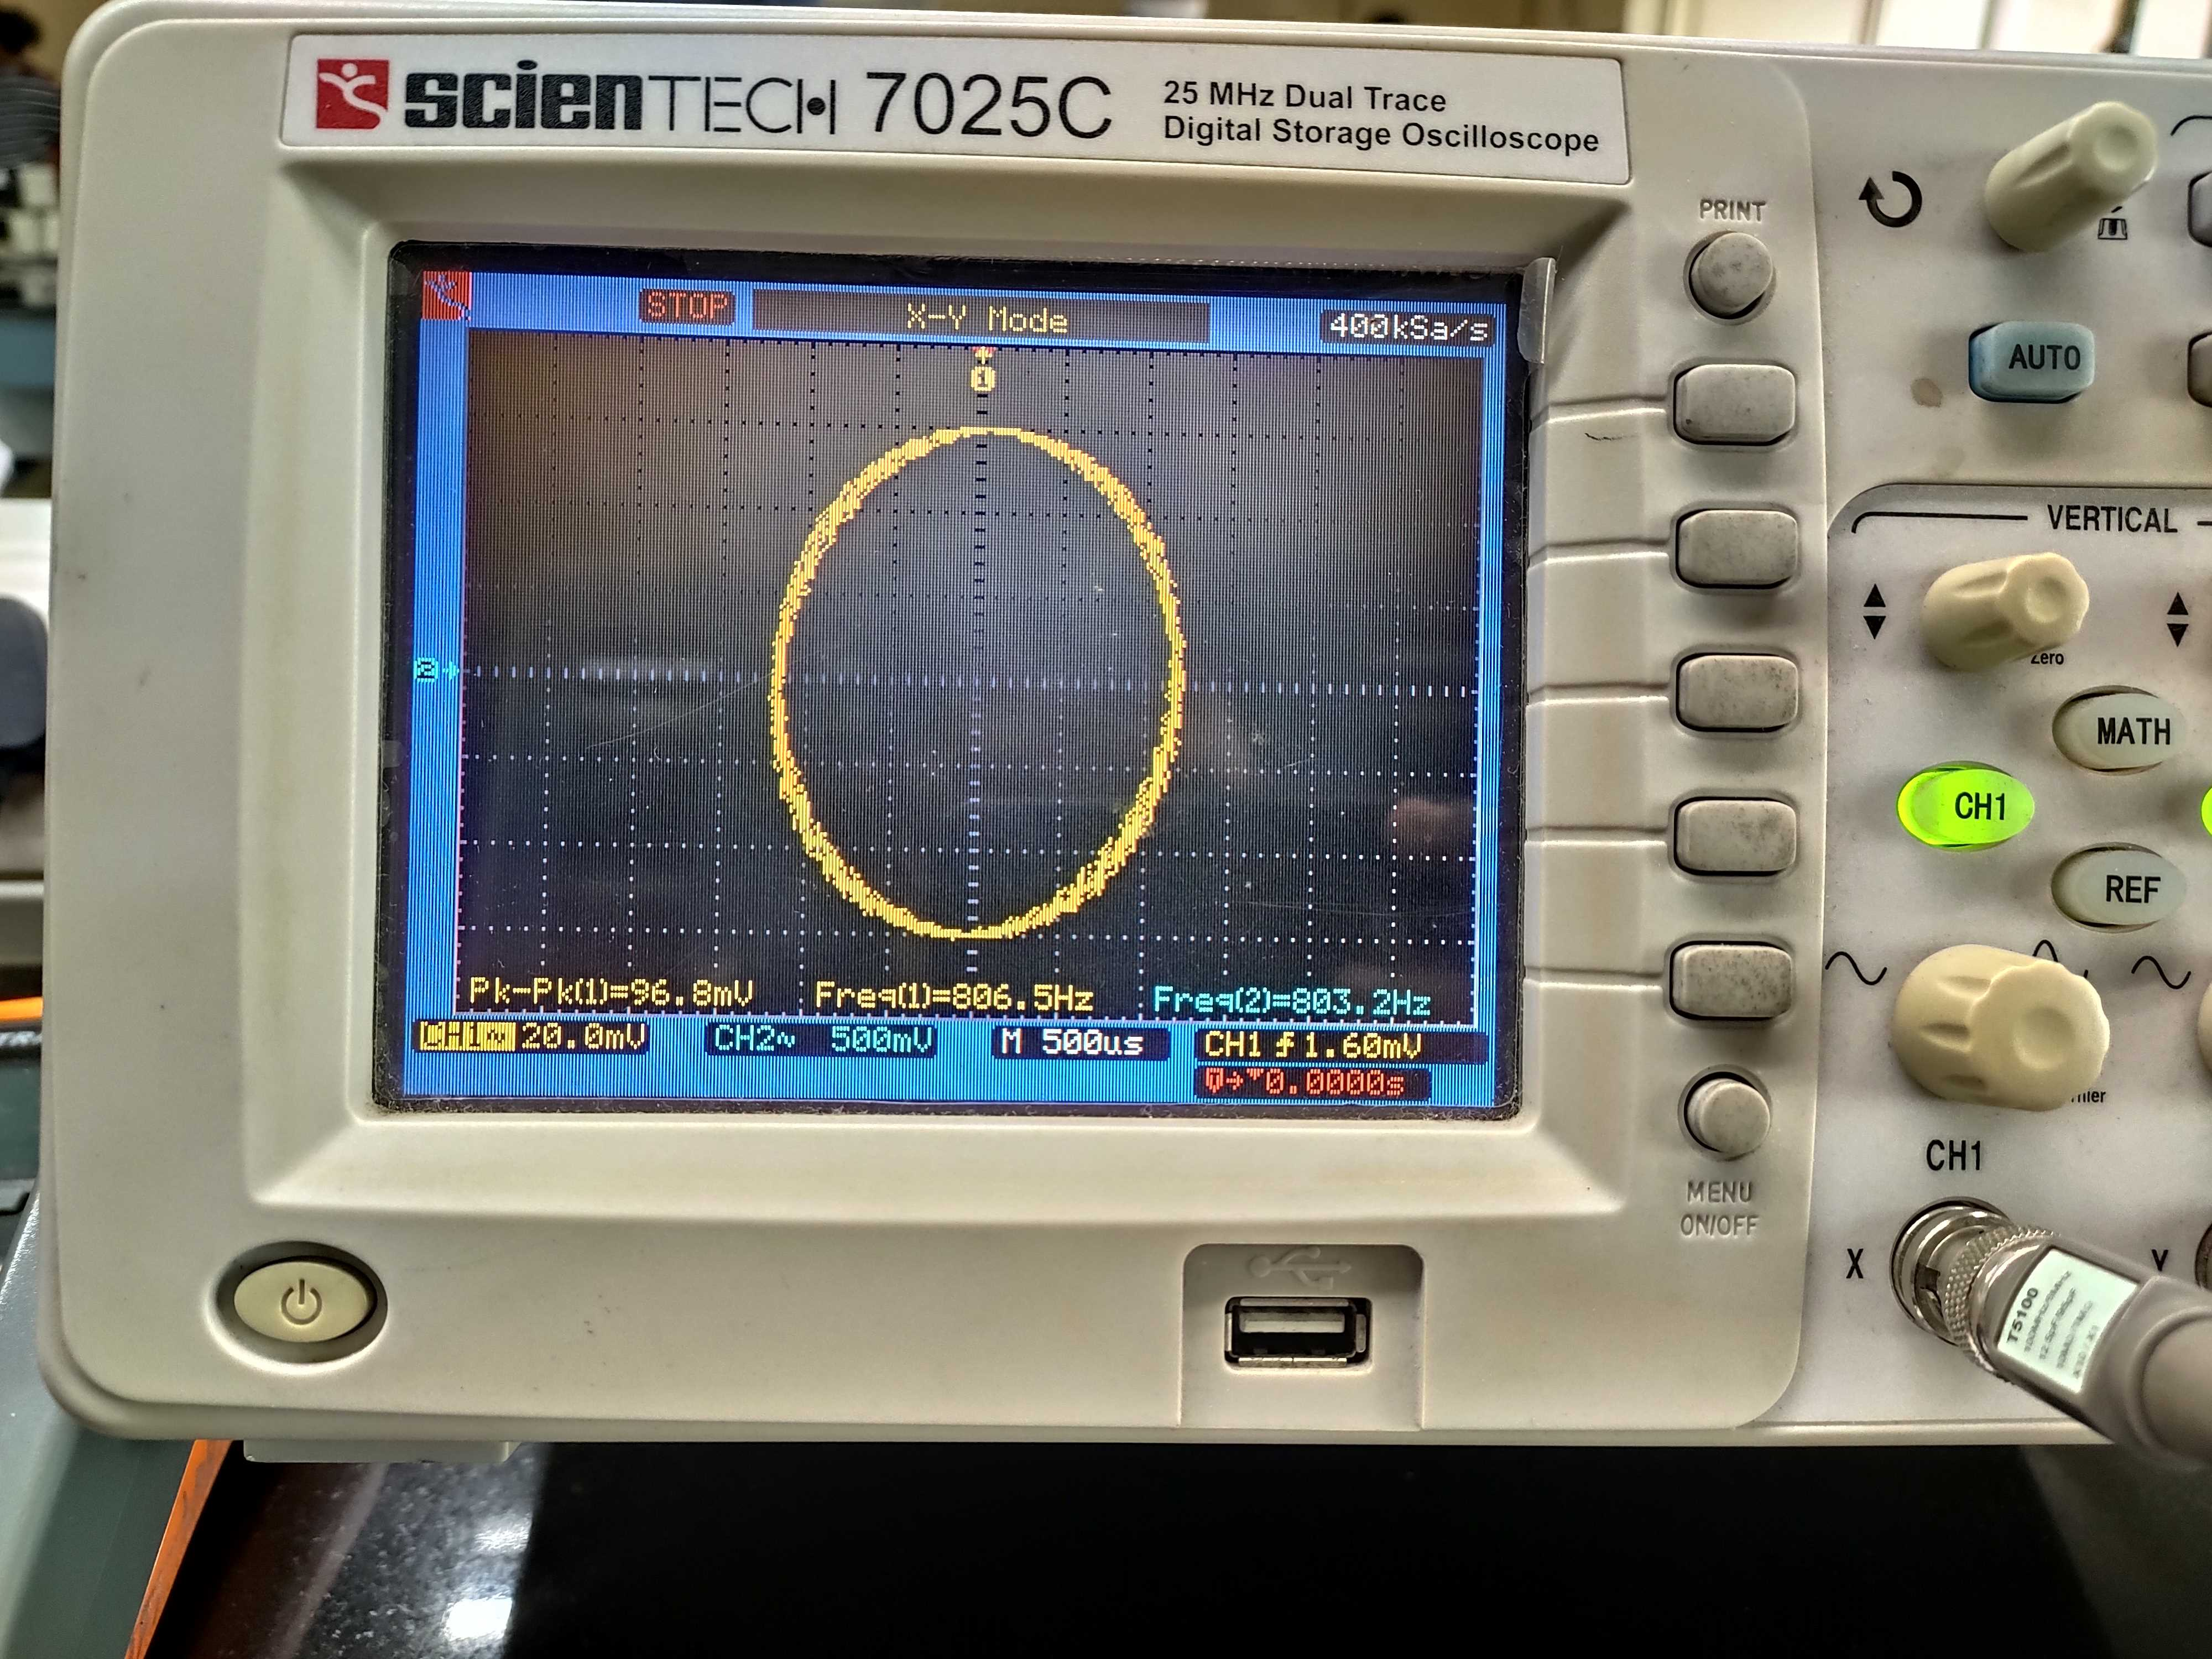
\includegraphics[scale = 0.11]{Documents/Lissajous.jpg}
\end{center}
\begin{center}
    \textbf{The Lissajous figure obtained from sustained oscillations}
\end{center}
\section{Results}
\begin{enumerate}
    \item The resonant frequency so obtained as the result of the experiment is $\SI{757.6}{\hertz}$.
    \item The Lissajous figure obtained resembles an ellipse.
\end{enumerate}
\section{Discussions}
\begin{enumerate}
    \item We observe that although some starting voltage is supplied to the oscillator circuit, but no signal is applied to the oscillator but still, the oscillations are obtained at the output.
    \item The origin of these oscillations can be attributed to the thermal noise generated due to the motion of charge carriers present in the conducting circuit. This thermal noise contains all the frequencies. 
    \item As soon as the oscillator is turned on, all these frequency components present in the thermal noise are amplified by the Op-Amp. This amplified output is then given as the input to the feedback circuit.
    \item This circuit is a frequency selective circuit so out of all frequencies present in the noise, only only will give the condition for resonance.
    \item The seemingly random factor of 29 can be explained using the general expression that is derived for the phase-shift oscillator circuit.
    \item As the feedback resistor has more than enough resistance, the oscillations could sustain themselves.
    \item The phase shift oscillator can used to generate the signals over an extensive range of frequency. So they are used in musical instruments, GPS units, and voice synthesis.
\end{enumerate}
\section{Error Analysis}
\begin{enumerate}
    \item The calculated resonant frequency for the phase-shift oscillator is $\SI{760.32}{\hertz}$. The frequency as obtained experimentally is $\SI{757.6}{\hertz}$. Therefore,
    \begin{center}
        Percentage error = $\dfrac{760.32-757.6}{760.32}\times 100 \% = 0.36\%$
    \end{center}
\end{enumerate}
\section{Conclusion}
\begin{enumerate}
    \item All results obtained are in accordance to the expectations.
    \item The errors are quite small and are due to elements of the circuit.
\end{enumerate}